

\section{Calibración}
\label{calibracion}

\subsection{Introducción}
Para poder obtener la posición en tres dimensiones de los marcadores a partir de las imágenes capturadas es necesario que las cámaras estén previamente calibradas. El objetivo de la calibración consiste en determinar un conjunto de parámetros tal que pueda establecerse una relación entre el espacio 3D y las coordenadas 2D de las imágenes.\\

Los puntos en el espacio pueden ubicarse respecto a un sistema de coordenadas 3D. A su vez, los puntos capturados en las imágenes pueden referenciarse respecto a un sistema de coordenadas 2D en píxeles. Si se quiere determinar la posición de un punto en el espacio en función de las correspondientes proyecciones de dicho punto en las imágenes capturadas por las cámaras, es necesario determinar las ecuaciones que vinculan al sistema de coordenadas del espacio con el sistema de coordenadas en píxeles de las cámaras.\\

De la relación entre estos sistemas de coordenadas se obtienen los parámetros de las cámaras. Dichos parámetros se clasifican en intrínsecos y extrínsecos. Los primeros son aquellos que describen las propiedades geométricas y ópticas de la cámara, es decir, las características internas de la cámara. Por otra parte, los parámetros extrínsecos son los que describen la posición y orientación de la cámara respecto al sistema de coordenadas del espacio.\\

Para realizar esto es necesario establecer un modelo que describa el sistema óptico de las cámaras. Esto es, el modelo por el cual una cámara es capaz de transformar el espacio 3D en imágenes de dos dimensiones. Un modelo simple y que describe estos sistemas adecuadamente es el modelo \textit{pinhole} de las cámaras. 
El modelo \textit{pinhole} se basa en la implementación mas simple de una cámara real, la cámara estenopeica. En dicha cámara la imagen capturada esta conformada por la proyección del espacio 3D a través de un punto situado delante de la retina de la cámara como se muestra en la figura \ref{pinhole_camara}. El modelo de esta cámara se describe en la figura \ref{pinhole_modelo}.\\

\begin{figure}[h!]
\begin{center}
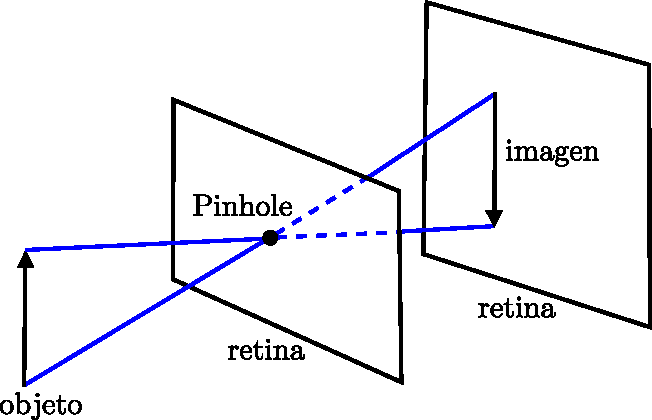
\includegraphics[scale=0.5]{img/calibracion/pinhole_camara}
\end{center}
\caption{Cámara estenopeica .\cite{faugeras_libro}}
\label{pinhole_camara}
\end{figure}



\begin{figure}[ht]
\begin{center}
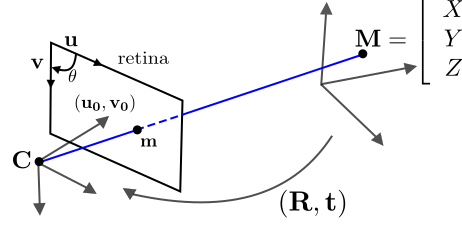
\includegraphics[scale=0.7]{img/calibracion/pinhole_modelo}
\end{center}
\caption{Modelo "pinhole" de una cámara.\cite{zhang_libro}}
\label{pinhole_modelo}
\end{figure}

En dicho modelo, una cámara se representa por un punto $C$, foco de la cámara, y un plano, al  que se le llama retina de la cámara. La imagen que se proyecta en la retina corresponde a la imagen capturada por la cámara. Dado un punto $M$ en el espacio, su correspondiente proyección en la retina, el punto $m$, se encuentra en la intersección de la retina y la recta formada por los puntos $C$ y $M$ de manera que $C$, $M$ y $m$ son colineales.\\ 




Si las coordenadas del punto  $M$ y las del punto $m$ son las siguientes:


\[m = \begin{bmatrix}
u \\ 
v
\end{bmatrix} , \quad
M = \begin{bmatrix}
X \\ 
Y \\
Z
\end{bmatrix} \]

Notando con $\tilde{x}$ a los vectores en coordenadas homogéneas se tiene:

% ANEXO EXPLICANDO COORDENADAS HOMOGÉNEAS??

\[\tilde{m} = \begin{bmatrix}
u \\ 
v \\
1
\end{bmatrix} , \quad
\tilde{M} = \begin{bmatrix}
X \\ 
Y \\
Z \\
1
\end{bmatrix} \]

Tomando el modelo \textit{pinhole} de la cámara, la relación entre un punto $M$ y su proyección $m$ es:
\begin{equation}
s\tilde{m} = A [R \quad t]\tilde{M}
\label{proyeccion}
\end{equation}




\begin{equation}
\text{siendo }
A = \begin{bmatrix}
\alpha & c & u_0 \\ 
0 & \beta & v_0 \\ 
0 & 0 & 1
\end{bmatrix} 
\end{equation}

Por lo tanto estos puntos se relacionan a través de la matriz $P = A [R \quad t]$, a menos de un factor de escala $s$. A dicha matriz  se le denomina Matriz de Proyección de la cámara.\\

La matriz $P$ se compone a su vez de la matriz $A$ que representa los parámetros intrínsecos de la cámara, y la matriz $[R \quad t]$ que representa los parámetros extrínsecos.\\

La matriz $[R \quad t]$ está formada por la rotación y traslación que relaciona el sistema de coordenadas del espacio con el sistema de coordenadas de la cámara. La matriz $A$ está formada por los parámetros intrínsecos de la cámara:\\



\begin{tabular}{cp{.8\textwidth}}


$(u_0, v_0)$ &  coordenadas del punto principal. \\ 
$\alpha$ y $\beta$ & factores de escala en los ejes de imagen  $u$ y $v$. \\ 
$c$ & grado de oblicuidad de los ejes imagen
\end{tabular} \\

El punto principal $(u_0, v_0)$ se define como el punto formado por la intersección de la retina y la recta perpendicular a dicha retina que pasa por el punto $C$. La distancia entre el punto $C$ y el punto principal se define como la distancia focal de la cámara $f$. Los factores $\alpha$ y $\beta$ se relacionan con la relación de aspecto de los píxeles de la cámara. El parámetro $c$ se relaciona con el ángulo $\theta$ formado por los ejes $u$ y $v$.\\

Por lo tanto la proyección de un punto 3D sobre la retina se compone de los siguientes pasos:\\

\begin{itemize}
\item Se pasa del sistema de coordenadas del espacio 3D $(X_w, Y_w, Z_w)$ al sistema de coordenadas de la cámara $(X,Y, Z)$
\begin{equation}
[X \ Y \ Z] = [X_w \ Y_w \ Z_w]^T + t
\end{equation}
\item Se proyecta el punto 3D respecto a las coordenadas de la cámara sobre las coordenadas imagen de la retina $(x,y)$.
\begin{equation}
x=f \dfrac{X}{Z} \qquad y = \dfrac{Y}{Z}
\end{equation}
\item En algunos casos puede ser necesario modelar además ciertas distorsiones introducidas por el lente de la cámara.
\begin{equation}
\check{x} = x + \delta_x \qquad \check{y} = y + \delta_y
\end{equation}

Siendo $(\check{x},\check{y})$ las coordenadas distorsionadas y $(\delta_x, \delta_y)$ las distorsiones aplicadas a $(x,y)$.

\item Por último se pasa de la coordenadas imagen $(\check{x}, \check{y})$ a las coordenadas en píxeles $(\check{u}, \check{v})$.

\begin{equation}
\check{u} + d_x ^{-1}\check{x} + u_0 \qquad \check{v} + d_y ^{-1}\check{y} + v_0
\end{equation}

Siendo $d_x$ y $d_y$ las distancias entre píxeles adyacentes en las direcciones horizontal y vertical, respectivamente.\\
\end{itemize}


\subsection{Métodos de calibración}

De acuerdo a los objetos utilizados para realizar la calibración, los métodos pueden clasificarse de la siguiente manera \cite{zhang_libro}:\\

\begin{itemize}
\item Calibración mediante objetos 3D\\

La calibración mediante este método es realizada capturando la imagen de un objeto de calibración cuyas dimensiones y geometría son conocidas. Los objetos de calibración suelen ser planos colocados ortogonalmente. También pueden utilizarse estructuras con marcadores de dimensiones conocidas. A estos objetos se les aplica traslaciones en el espacio logrando más cantidad de puntos de referencia para calibrar. La ventaja de este método es su precisión aunque se requiere de objetos más costosos y procedimientos más elaborados.\\

\item Calibración mediante objetos 2D\\

Este caso se utiliza objetos planos con figuras de patrones determinados, por ejemplo dameros. Estos objetos son colocados en varias posiciones delante de la cámara de manera de capturar varias imágenes del objeto. Esta metodología ofrece más flexibilidad para calibrar.\\

\item Auto calibración\\

Este método consiste en obtener la información necesaria a través de la captura de varias imágenes de un escena estática, prescindiendo de objetos para calibrar. Esta método es más flexible que  los anteriores aunque suele ser menos preciso.\\

\end{itemize}


Algunas soluciones comerciales, como por ejemplo Vicon \footnote{\textcolor{blue}{\underline{\url{http://www.vicon.com}}. Accedido 3-12-14.}} , utiliza como objeto de calibración una vara con leds, ver figura \ref{vicon}. 

\begin{figure}[H]
        \centering
        
        \subfloat{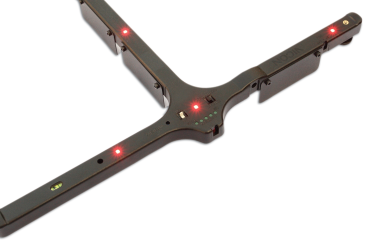
\includegraphics[scale=1.8]{img/calibracion/vicon1.png}}
        \hspace{1.8cm}
        \subfloat{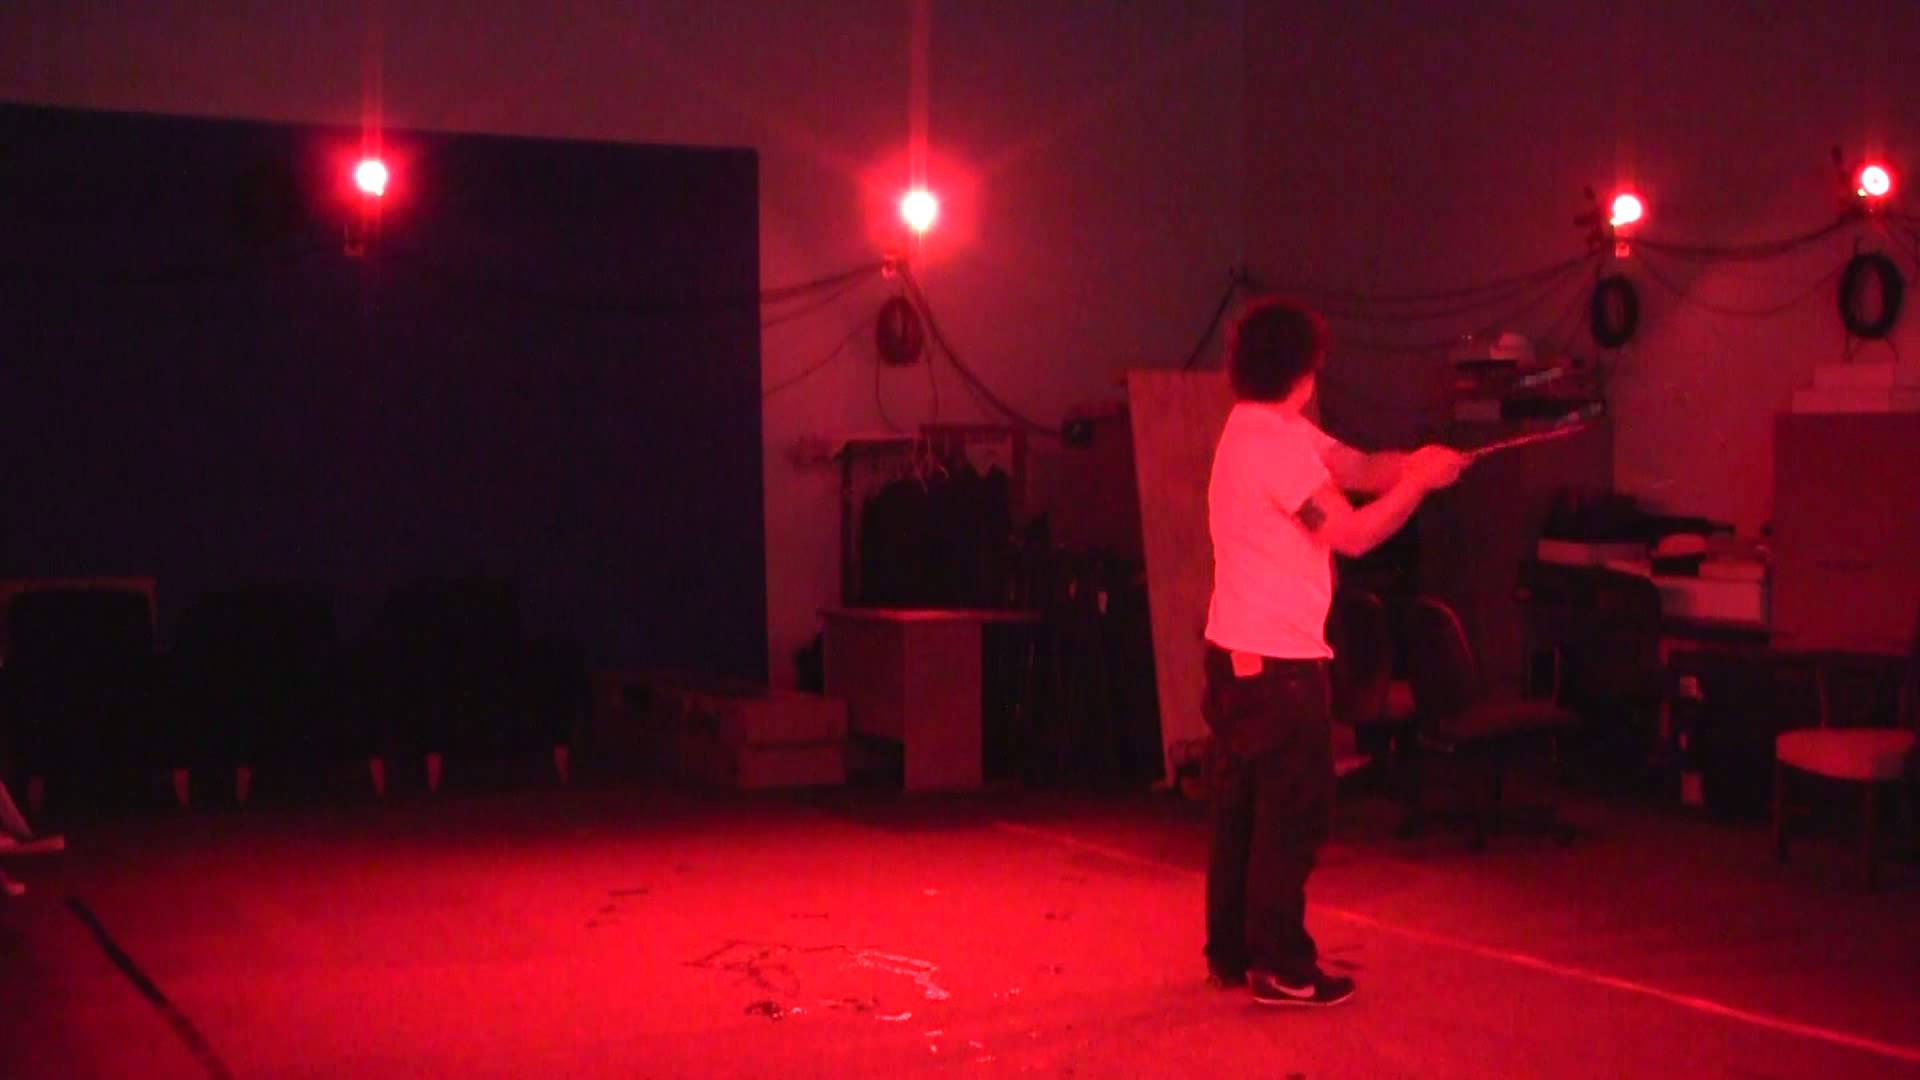
\includegraphics[scale=0.08]{img/calibracion/vicon2.jpg}}
  \caption{Calibración Vicon}
      \label{vicon}
\end{figure}

En este caso la calibración se realiza moviendo el objeto de calibración a través del espacio de trabajo. Este método resulta muy flexible para la calibración de un conjunto de varias cámaras simultáneamente.


\subsection{Calibración en el entorno Blender}

Una vez establecida la configuración de las cámaras en  Blender, según lo descrito en la sección \ref{section_base_de_datos}, es posible conocer las matrices de proyección de cada una de ellas a través de la información proporcionada por el propio programa de ciertos parámetros de las cámaras. Esto permite tener la calibración \textit{real} de las cámaras con lo cual es posible medir el desempeño de algunos bloques del sistema.\\

Si se conocen las coordenadas de un punto 3D en el espacio de trabajo de Blender y además se saben las matrices de proyección de las cámaras, es posible determinar las coordenadas 2D de dicho punto proyectado en cada una de las cámaras. De esta manera se tiene el \textit{ground truth} de la detección de marcadores, permitiendo comparar el desempeño de dicho bloque respecto  a la posición real de los marcadores en las vistas 2D. Análogamente teniendo estos datos se pueden evaluar los bloques siguientes del sistema. Por ejemplo, es posible además evaluar el desempeño del bloque de reconstrucción sabiendo la posición 2D real de los marcadores, por lo cual se puede evaluar los errores que son producto solamente de este bloque del sistema.\\

A continuación se describe cómo se deducen las matrices de proyección a partir de ciertos parámetros proporcionados por el programa.\\

La posición de una cámara se establece respecto a un sistema de coordenadas determinado, al que se le puede llamar el sistema de coordenadas del mundo. Por lo cual es posible saber la rotación y traslación que es necesario aplicar al sistema de coordenadas del mundo para obtener el sistema de coordenadas solidario a la cámara. Los parámetros que se pueden obtener de Blender son los ángulos de rotación $(\theta, \phi, \psi )$ respecto a los ejes $(x,y, z)$ del sistema de coordenadas del mundo, así como el orden en que se ejecutan dichas rotaciones. Si el orden establecido es \textit{XYZ Euler}, lo que implica que primero se rota respecto al eje $x$, luego al $y$ y al $z$, se obtiene la matriz de rotación:

\[R=R_{(z,\psi)}R_{(y,\phi)}R_{(x,\theta)}
= \begin{pmatrix}
		r_{11} & r_{12} & r_{13}\\
		r_{21} & r_{22} & r_{23}\\
		r_{31} & r_{32} & r_{33}\\ 
\end{pmatrix}= 
\begin{pmatrix}
			R_1 \\
			R_2 \\
			R_3 \\
		\end{pmatrix}
\]
 
 Donde,
 \[R_{(x,\theta)} = \begin{pmatrix}
		1 &   0         &  0\\
		0 & cos\,\theta & -sen\,\theta\\
		0 & sen\,\theta & cos\,\theta\\ 
\end{pmatrix}, ~
R_{(y,\phi)}=\begin{pmatrix}
		cos\,\phi  & 0 & sen\,\phi\\
		0          & 1 & 0\\
		-sen\,\phi &0  & cos\,\phi\\ 
\end{pmatrix}, ~
R_{(z,\psi)}\begin{pmatrix}
		cos\,\psi & -sen\,\psi & 0\\
		sen\,\psi & cos\,\psi  & 0\\
		 0          & 0            & 1\\ 
\end{pmatrix}\]

A su vez también es posible obtener el vector de traslación $T$ que es necesario aplicar al sistema de coordenadas del mundo para obtener el sistema solidario a la cámara. De esta manera se obtiene la matriz de parámetros extrínsecos:
\[
		M_{ext}=\begin{pmatrix}
			r_{11} & r_{12} & r_{13} &-R^t_1 T\\
			r_{21} & r_{22} & r_{23} &-R^t_2 T\\
			r_{31} & r_{32} & r_{33} &-R^t_3 T\\
		\end{pmatrix}
\] 

Para hallar la matriz de parámetros intrínsecos se necesitan saber los siguientes parámetros que son proporcionados por Blender: 
\begin{itemize}
\item $f$, distancia focal
\item $(o_x, o_y)$, coordenadas del punto principal
\item $(s_x,s_y)$, tamaño efectivo de los píxeles de la retina en píxeles/milímetro.
\end{itemize}

con estos parámetros se obtiene la matriz de parámetros intrínsecos:

\[M_{int}=\begin{pmatrix}
			-f/s_x & 0      & o_x\\
			0      & -f/s_y & o_y\\
			0      & 0      & 1\\
		\end{pmatrix} \]
 
%%%%%%%%APÉNDICE%%%%%%%%%%%%%%%%%%%55
%En el apéndice \ref{apendice_calibracion_blender} se describe en detalle cómo se obtienen los parámetros necesarios en Blender.\\

\subsection{Calibración para secuencias reales}

\label{seccion_calibracion_secuencias_reales}

%%%%%%%%%%%%REFERENCIAS%%%%%%%%%%%%%%%%%
% LIC DARIO SANTOS, HOSPITAL DE CLÍNICAS

Por intermedio del Lic. Darío Santos, hemos podido tener acceso a secuencias de vídeo de análisis del movimiento de la marcha que se han realizado en el Hospital de Clínicas. Dichas secuencias han sido obtenidas por un grupo de médicos e investigadores con el objetivo de analizar el movimiento de pacientes, es decir, con fines terapéuticos o con un objetivo esencialmente de investigación, en particular del estudio de la marcha humana desde el punto de vista de la biomecánica.\\

%DEBERÍA ACLARARSE QUE ESTO SE HACIA ANTES, CREO QUE TIPO POR 2009 Y AHORA USAN VICON.

La metodología utilizada consiste en el uso de tres cámaras de vídeo convencionales de 25 fps y resolución  720 x 576 píxeles. Dichas cámaras se disponen como se muestra en la figura \ref{fig: lab_real}, alrededor de una alfombra o cinta sobre la que se le pide al paciente que camine.


\begin{figure}[ht]
\begin{center}
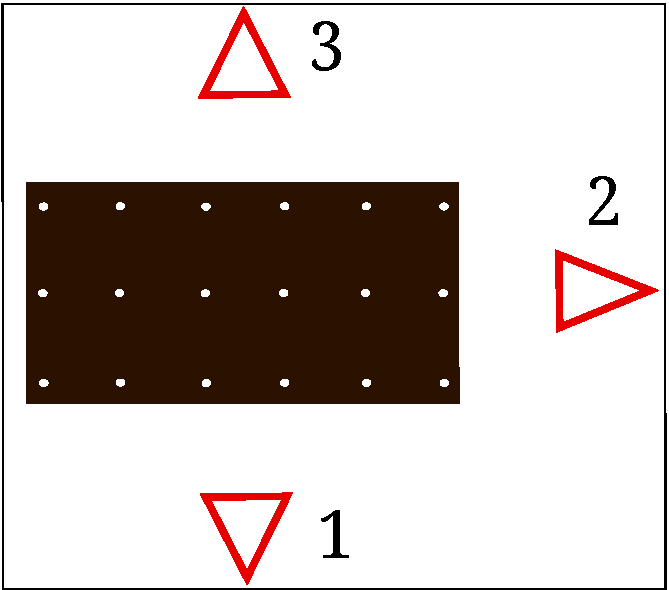
\includegraphics[scale=0.5]{img/calibracion/lab_real.pdf}
\end{center}
\caption{Laboratorio del Hospital de Clínicas}
\label{fig: lab_real}
\end{figure}

La persona que se desea evaluar debe tener colocados marcadores, fundamentalmente en las articulaciones del cuerpo, y debe desplazarse sobre la alfombra dispuesta para esto. En la figura \ref{fig: persona con marcadores}, se observa a un individuo caminando con los marcadores colocados.

\begin{figure}[H]
        \centering
        
        \subfloat[Persona con marcadores]{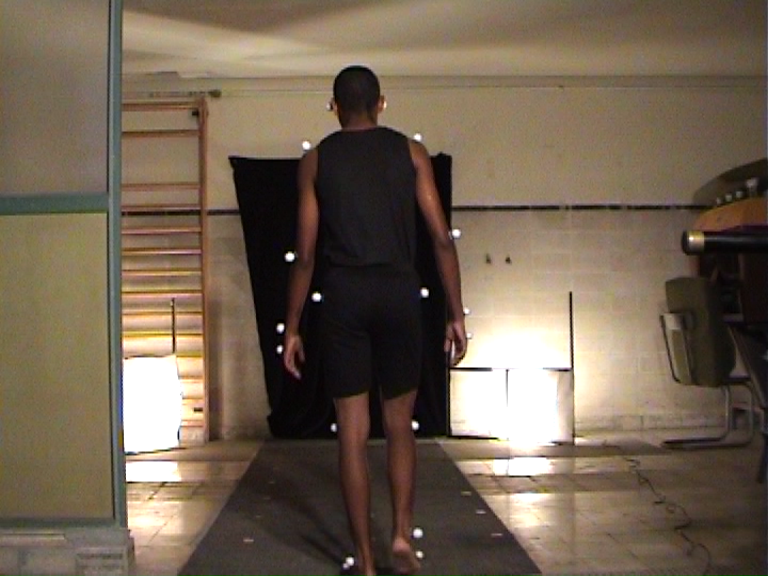
\includegraphics[scale=0.3]{img/calibracion/captura_real.png}\label{fig: persona con marcadores}}
        \hspace{0.2cm}
        \subfloat[Objeto de calibración]{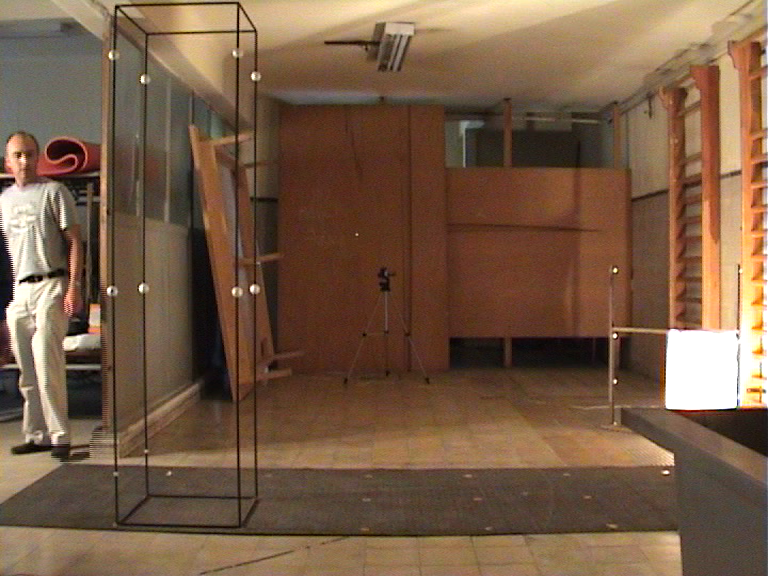
\includegraphics[trim = 20mm 0mm 40mm 0mm, clip, scale=0.3]{img/calibracion/calibrador.png}\label{fig: calibrador}}
  \caption{Captura de secuencia real}
      \label{fig: captura real}
\end{figure}

Antes de la captura del movimiento se emite una señal acústica con la cual se sincronizan las tres vistas una vez obtenidos los vídeos. El software con el cual este grupo de médicos han analizado el movimiento es el \textit{Dvideow}.            
 %%%%%%%%%%%%%%%%%%(REFERENCIAR)%%%%%%%%%%%%%%%%%%%%%%%%%%%%%%. 
 Dicho software realiza la detección, seguimiento y reconstrucción de los marcadores. No hemos podido tener acceso a este software por lo cual tampoco pudimos evaluar su desempeño y compararlo con el desarrollado por nosotros.\\

Para calibrar este sistema se utiliza el objeto de calibración, o calibrador, como se muestra en la figura \ref{fig: calibrador} que consiste en marcadores colocados sobre una estructura de dimensiones conocidas. Dicho objeto se coloca sobre distintos puntos marcados sobre la alfombra, por lo que las traslaciones realizadas son de distancias conocidas. De esta manera se calibra con más puntos sobre el volumen de trabajo.\\


El método implementado requiere que cada marcador del calibrador, en cada una de las vistas, sea seleccionado manualmente en un orden tal que permita establecerse una correspondencia entre las proyecciones de un mismo marcador en las tres vistas. En la figura \ref{fig: vistas_calibrador} se muestra a uno de los marcadores seleccionado en cada una de las vistas.\\


\begin{figure}[H]
        \centering        
        \subfloat[Vista cámara 1]{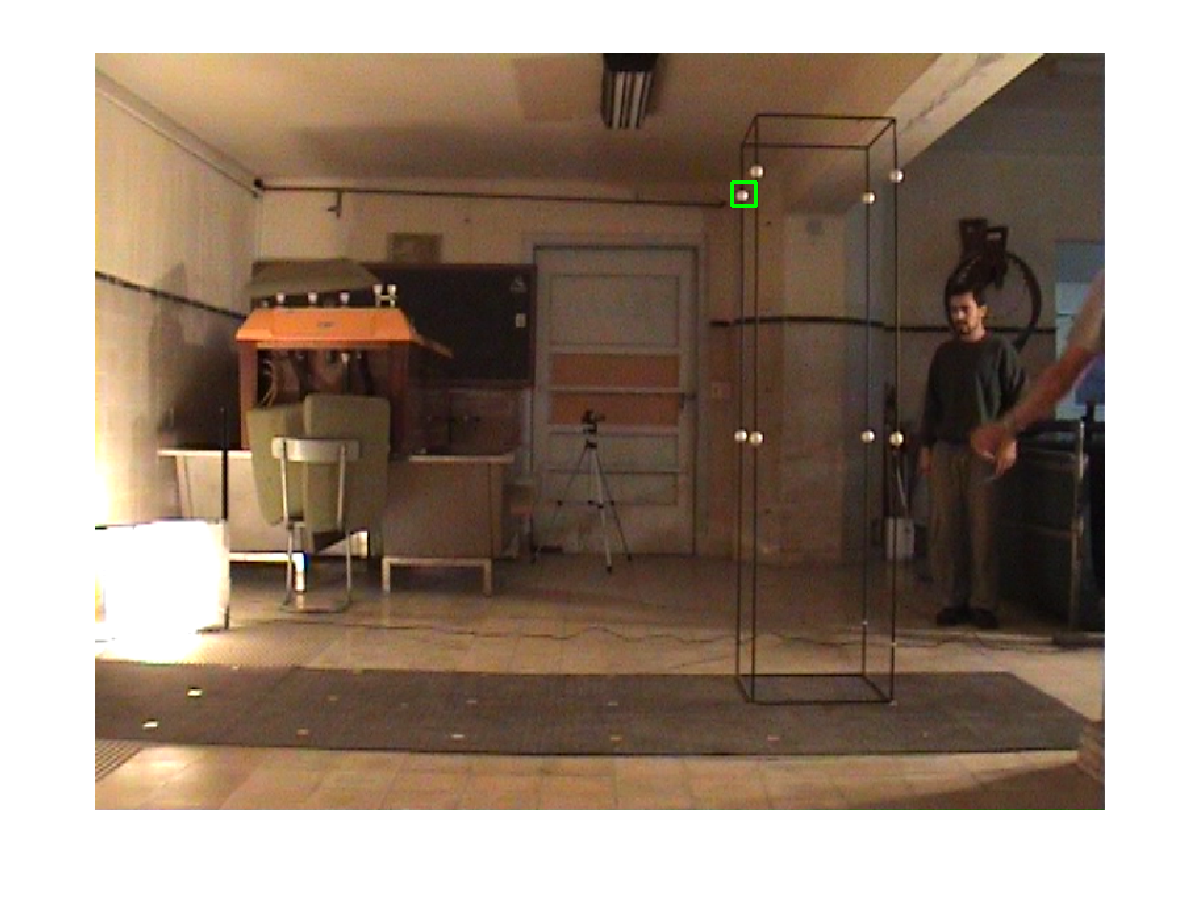
\includegraphics[trim = 59mm 0mm 41mm 0mm, clip,scale=0.47]{img/calibracion/calibrador_cam1.png}}
                \hspace{0.1cm}
        \subfloat[Vista cámara 2]{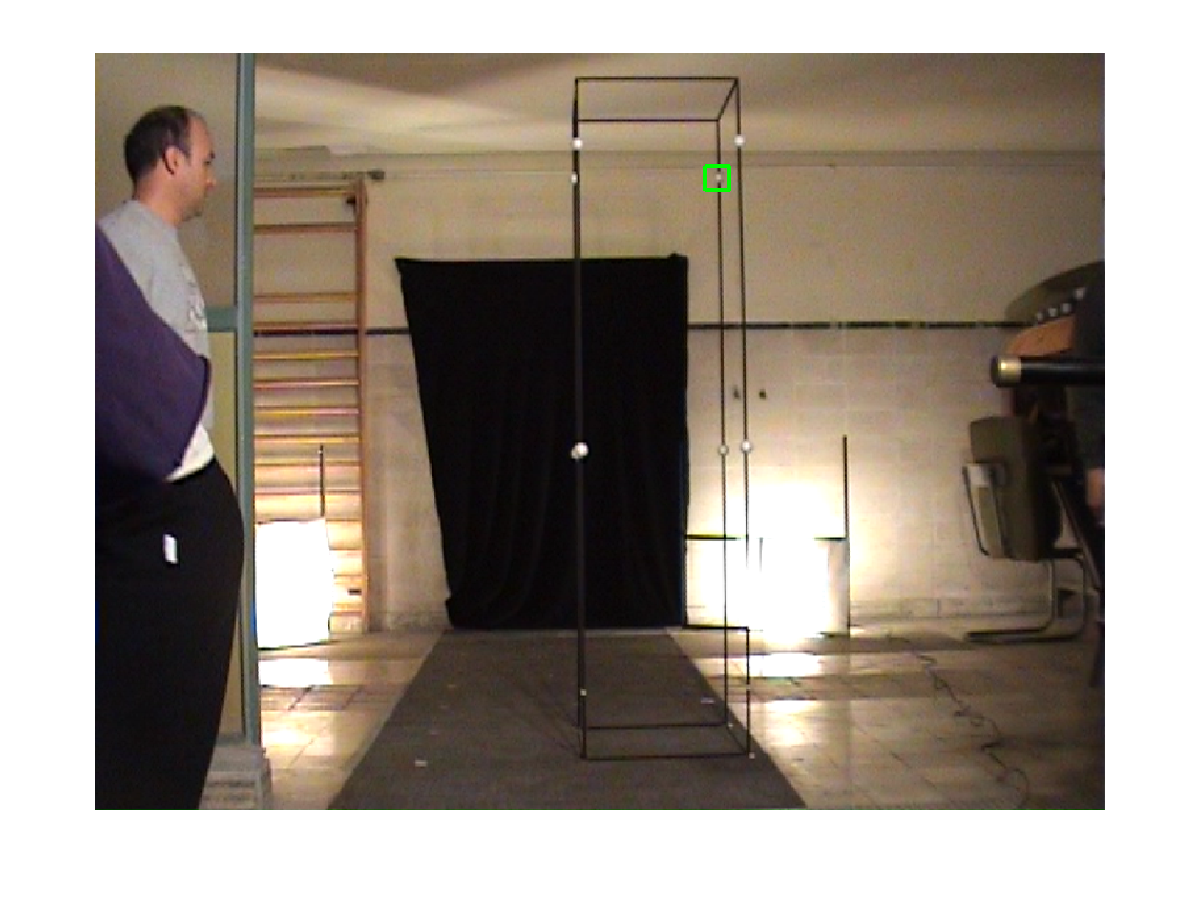
\includegraphics[trim = 50mm 0mm 50mm 0mm, clip,scale=0.47]{img/calibracion/calibrador_cam2.png}}     	
  \hspace{0.1cm}
        \subfloat[Vista cámara 3]{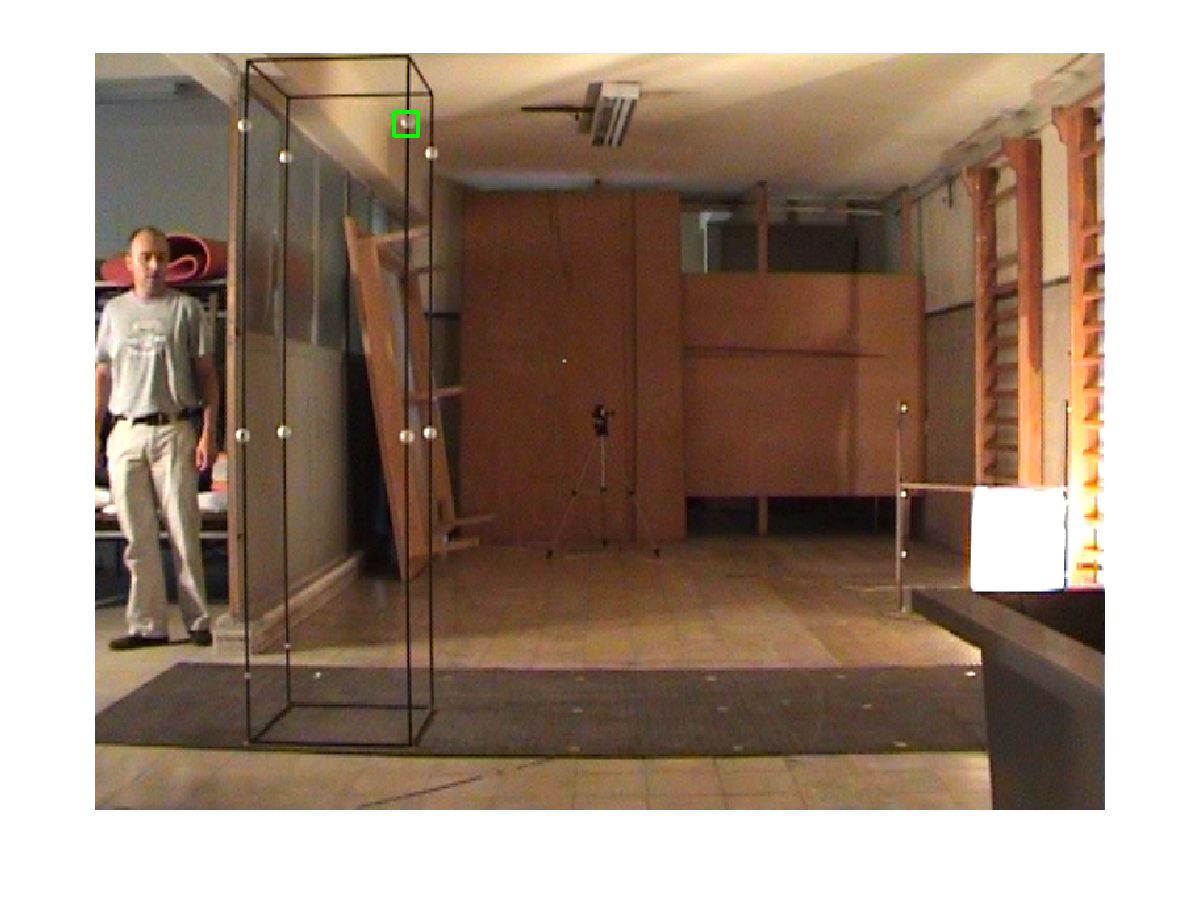
\includegraphics[trim = 32mm 0mm 68mm 0mm, clip,scale=0.47]{img/calibracion/calibrador_cam3.png}}
      
      \caption{Uno de los marcadores de calibrador seleccionado en cada una de las cámaras}
      \label{fig: vistas_calibrador}
      
\end{figure}


Por otra parte la posición de los marcadores en el espacio 3D es conocida ya que se saben las medidas del calibrador, ver figura \ref{fig: medidas_calibrador}. Dichas posiciones pueden ser referidas un punto que puede elegirse arbitrariamente, así como los ejes de coordenadas $(x,y,z)$.

\begin{figure}[H]
        \centering
     {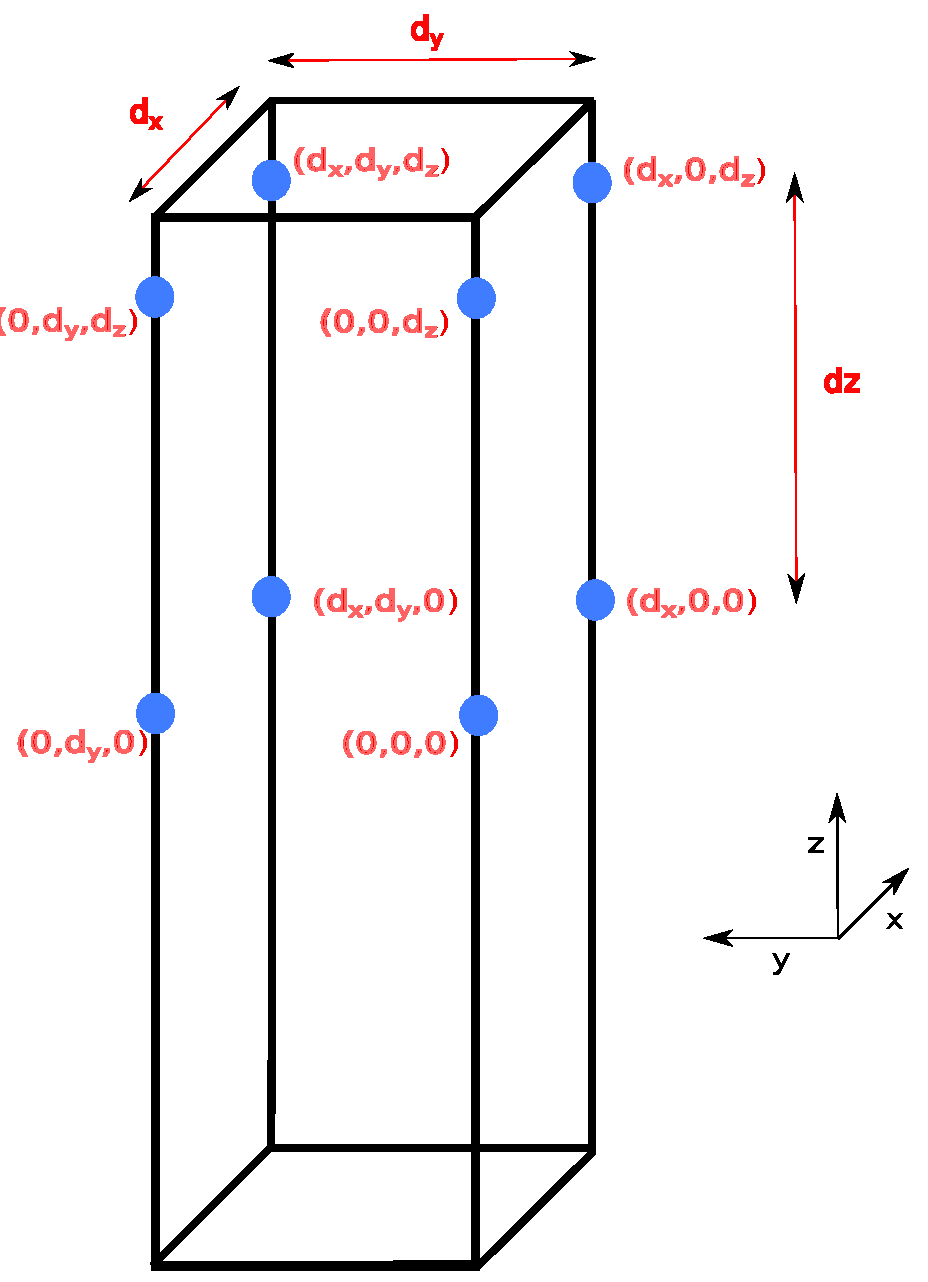
\includegraphics[scale=0.4]{img/calibracion/medidas_calibrador.pdf}}
    
     \caption{Coordenadas de los marcadores del calibrador}
      \label{fig: medidas_calibrador}     
\end{figure}

   De esta forma se tiene asociados las coordenadas 3D de los marcadores en el espacio con sus correspondientes coordenadas 2D en píxeles en cada una de las cámaras, $X_i \leftrightarrow x_i$. Si se tiene una cantidad suficiente de puntos, entonces las matrices de proyección $P$ pueden ser estimadas tal que $x_i=PX_i$. Para esto se utiliza el algoritmo \textit{DLT}.\\
   
   Para cada asociación de puntos $X_i \leftrightarrow x_i$ se cumple que \cite{hartley}:
   
   \[
   \begin{pmatrix}
   0^T & -w_iX_i^T & y_iX_i^T \\
   w_iX_i^T & 0^T & -x_iX_i^T
   \end{pmatrix}
   \begin{pmatrix}
    P^1 \\
    P^2 \\
    P^3
   \end{pmatrix}
   = 0
   \]
   
 siendo $P^{iT}$ las columnas $i$-ésimas de $P$. Dicha matriz se obtiene resolviendo un conjunto de ecuaciones del tipo $Ap=0$.  Dado que por cada punto se tiene 2 ecuaciones y que la matriz $P$ tiene 12 entradas y 11 grados de libertad, ignorando el factor de escala, resulta que son necesarios conocer al menos 6 correspondencias $X_i \leftrightarrow x_i$.\\
 
 Tanto a los puntos imagen 2D como a los 3D se les aplica una normalización. Para los puntos 2D de cada vista se traslada el origen de coordenadas de dicha vista al centroide de los puntos y se aplica un escalado tal que la distancia promedio de los puntos al origen sea $\sqrt{2}$. Para los puntos 3D el mismo procedimiento excepto que el escalado que se aplica es tal que la distancia promedio al origen es $\sqrt{3}$. De esta manera se tiene dos matrices que realizan esta transformación, la matriz $T_{3D}$ tal que $\tilde{X_i} = T_{3D}^{}X_i$ para los puntos en el espacio, siendo $\tilde{X_i}$ los puntos normalizados. Análogamente para los 2D imagen se tiene la matriz $T_{2D}^{}$ tal que $\tilde{x_i} = T_{3D}^{}x_i$. \\
 
 Dado que las coordenadas de los puntos 2D están afectadas por el ruido y que se tienen más de 6 correspondencias $X_i \leftrightarrow x_i$ no existe una solución exacta a las ecuaciones $Ap=0$. Por lo tanto la solución se obtiene minimizando un error, en este se busca $p$ tal que minimice $||Ap||$. Para esto se utiliza la descomposición en valores singulares (SVD), donde se obtiene del vector singular asociado al menor valor singular. De esta manera se obtiene la matriz de proyección $\tilde{P}$. Por último debe descomponerse la normalización, por lo tanto la matriz de proyección $P = T_{2D}^{-1} \tilde{P} T_{3D}^{}$.
 
 \subsection{Calibración simulada en Blender}
 
 Con el objetivo de establecer una metodología que fuera válida para la configuración de cámaras con las que se diseño la base de datos, se probaron implementaciones existentes que pudieran calibrar dicha base de datos elaborada en Blender. Para esto se evaluó el siguiente toolbox elaborado en Matlab.\\ 
 
  \subsubsection{Toolbox Multi-Camera Self-Calibration \footnote{\textcolor{blue}{\underline{http://cmp.felk.cvut.cz/~svoboda/SelfCal/}. Accedido 3-12-14.}}}
 
 Este toolbox está especialmente pensado para la calibración simultánea de un conjunto de varias cámaras. El procedimiento consiste en capturar con todas las cámaras, el movimiento de una fuente puntual de luz que se mueve a lo largo de todo el volumen de trabajo. por tanto para cada cuadro se tiene un punto 3D en el espacio en una posición distinta y en cada una de las cámaras su correspondiente proyección si dicho punto es visible desde esa cámara. Para esto debe asegurarse que exista un contraste suficiente de la luz respecto al laboratorio. Puede usarse para esto, por ejemplo una lámpara led y que en el laboratorio exista poca o nula luz ambiente.\\
 
 
 Si se tienen $m$ cámaras y $n$ puntos 3D  
$\mathbf{X_j} = [X_j, Y_j, Z_j,1]^T$ con $j=1,\ldots,n$. La proyección de dichos puntos en los puntos imagen $u_j^i$:
\[ \lambda_j^i
\begin{bmatrix}
u_j^i \\
v_j^i \\
1
\end{bmatrix} 
 = \lambda_j^i u_j^i = P^i \mathbf{X_j}
\]

siendo $P^i$ la matriz de proyección de la $i$-ésima cámara y $u,v$ las coordenadas en píxeles de los puntos imagen. Las coordenadas de dichas proyecciones deben ser detectadas para cada cuadro y para cada cámara. El objetivo de la calibración es hallar los factores de escala $\lambda_j^i$ y las matrices de proyección $P^i$. Pueden expresarse todos los puntos y las matrices de proyección en una sola matriz $W_s$:

\[
W_s =
\begin{bmatrix}

	\lambda_1^1
	\begin{bmatrix}
	u_1^1 \\
	v_1^1 \\
	1
	\end{bmatrix} &
	
	\ldots &
	
	\lambda_n^1
	\begin{bmatrix}
	u_n^1 \\
	v_n^1 \\
	1
	\end{bmatrix} \\
	
	\vdots & \ddots & \vdots \\
	
	
	\lambda_1^m
	\begin{bmatrix}
	u_1^m \\
	v_1^m \\
	1
	\end{bmatrix} &
	
	\ldots &
	
	\lambda_n^m
	\begin{bmatrix}
	u_n^m \\
	v_n^m \\
	1
	\end{bmatrix} \\

\end{bmatrix}
= 
\begin{bmatrix}
P^1 \\
\vdots \\
P^m
\end{bmatrix}_{3m\text{x}4}
\quad
[\mathbf{X_1} \ldots \mathbf{X_n}]_{4\text{x}n}
\]
Por lo tanto se puede expresar:
\[ W_s = PX\]

donde $P = [P^1 \ldots P^m]^T$ y $X = [\mathbf{X_1} \ldots \mathbf{X_n}]$

Si son detectados una cantidad suficiente de puntos no ruidosos ($u_j^i, v_j^i$) y se conocen los $\lambda_j^i$, entonces $W_s$ tiene rango 4  y se puede factorizar en $P$ y $X$.\\

El número mínimo de cámaras para una correcta calibración depende del número de parámetros conocidos de las cámaras o del número de parámetros que se conocen pero son los mismos para todas las cámaras. 3 cámaras son suficientes si se conocen todos los puntos principales o si los parámetros internos de las cámaras no se conocen pero son los mismo para todas ellas.\\

La simulación en Blender se logra creando un punto 3D que toma para cada cuadro distintas posiciones en forma aleatoria dentro del volumen de trabajo. Para cada cuadro se \textit{renderiza} su posición en las 17 cámaras. En este caso se han tomado 500 posiciones distintas. En la figura \ref{fig: blender toolbox laser} se muestra en Blender la distintas posiciones que toma en un punto dentro del volumen de trabajo.

\begin{figure}[ht]
\begin{center}
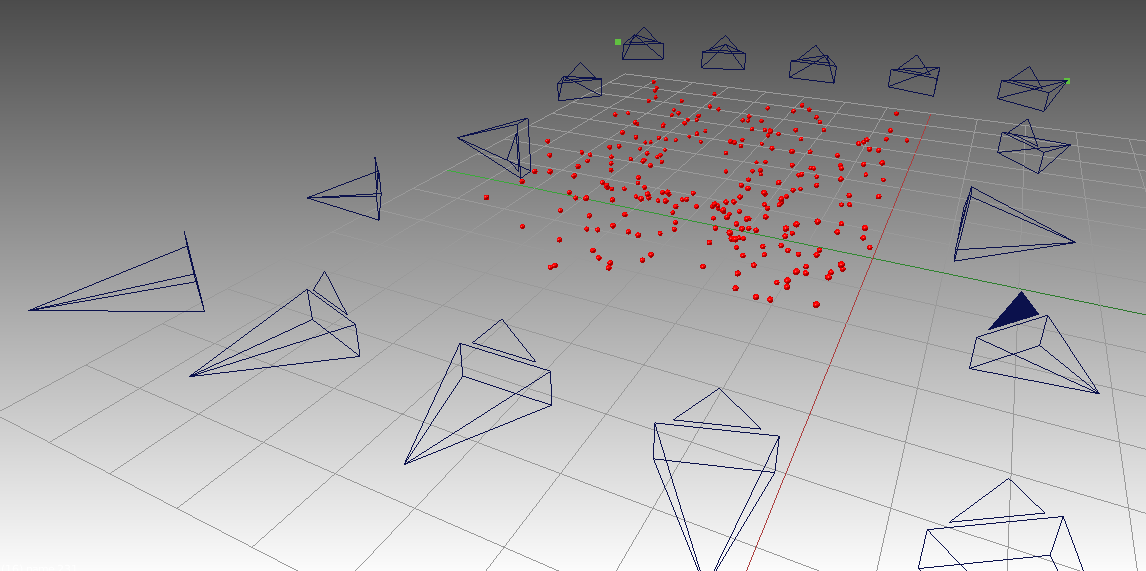
\includegraphics[scale=0.22]{img/calibracion/blender_toolbox_laser.png}
\end{center}
\caption{Posiciones de un punto 3D dentro del volumen de trabajo}
\label{fig: blender toolbox laser}
\end{figure}

En la figura \ref{fig: camaras blender} se muestra la configuración de las 17 cámaras en el espacio 3D de Blender. En la figura \ref{fig: camaras calibracion} se muestra, con círculos en azul, la posición de las cámaras obtenidas del resultado de la calibración. Se observa además, en rojo, la reconstrucción de las posiciones del punto 3D en el espacio.


\begin{figure}[H]
        \centering        
        \subfloat[Blender]{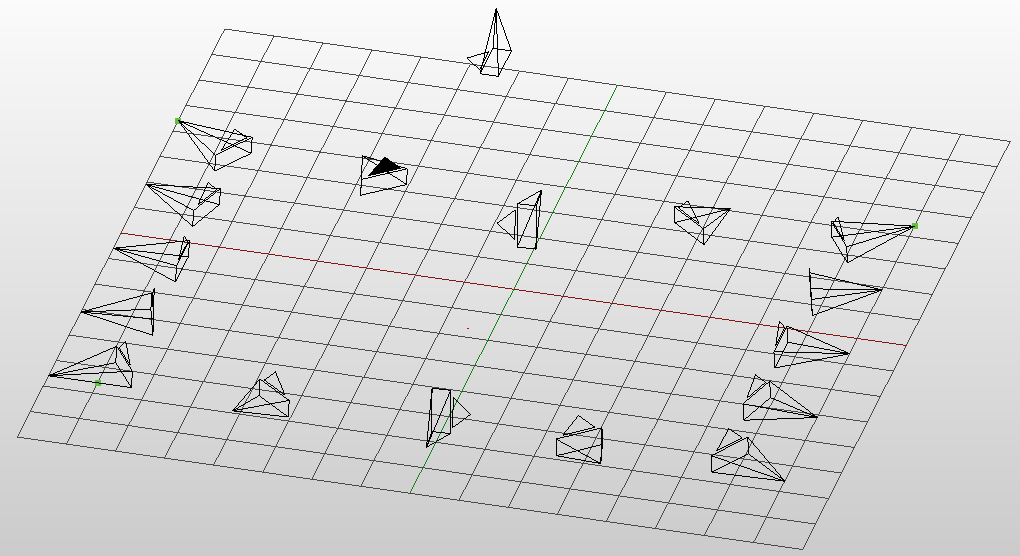
\includegraphics[trim = 0mm 0mm 0mm 0mm, clip,scale=0.25]{img/calibracion/camaras_blender.png}\label{fig: camaras blender}}
                \hspace{0.1cm}                
        \subfloat[Calibración]{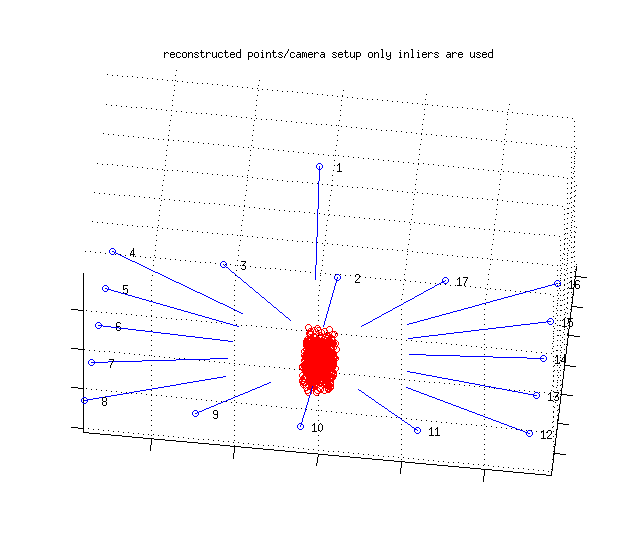
\includegraphics[trim = 0mm 20mm 10mm 20mm, clip,scale=0.47]{img/calibracion/camaras_calibracion.png}\label{fig: camaras calibracion}}
        
      
      \caption{Configuración de las cámaras en el espacio 3D de Blender y la misma configuración hallada mediante la calibración}
      \label{fig: configuracion camaras}
      
\end{figure}

En la figura \ref{fig: error reproyeccion} se muestra e promedio y la desviación del error de re-proyección estándar obtenido para cada una de las cámaras.

\begin{figure}[ht]
\begin{center}
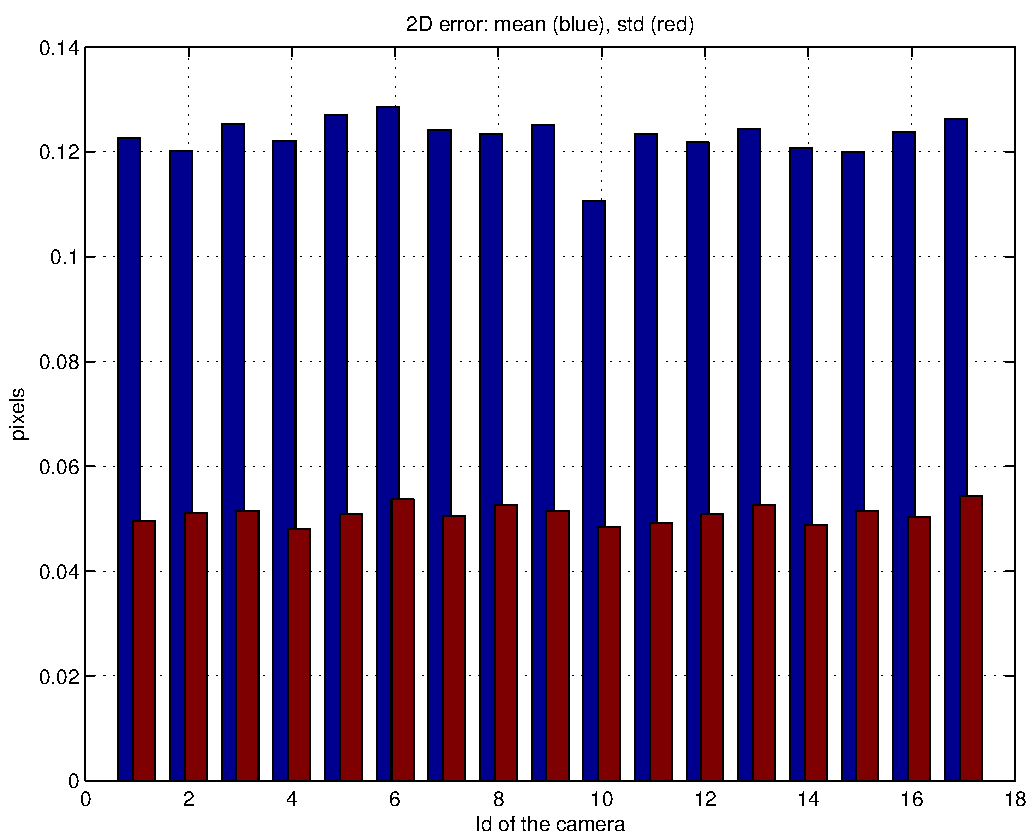
\includegraphics[scale=0.4]{img/calibracion/reprerrors.pdf}
\end{center}

\caption{Promedio y desviación  del error de re-proyección en todas las cámaras }
\label{fig: error reproyeccion}
\end{figure}
  






